\documentclass[border=5mm]{standalone}
\usepackage{tikz}
\usetikzlibrary{arrows.meta,positioning,calc}
\usepackage{times}

\begin{document}
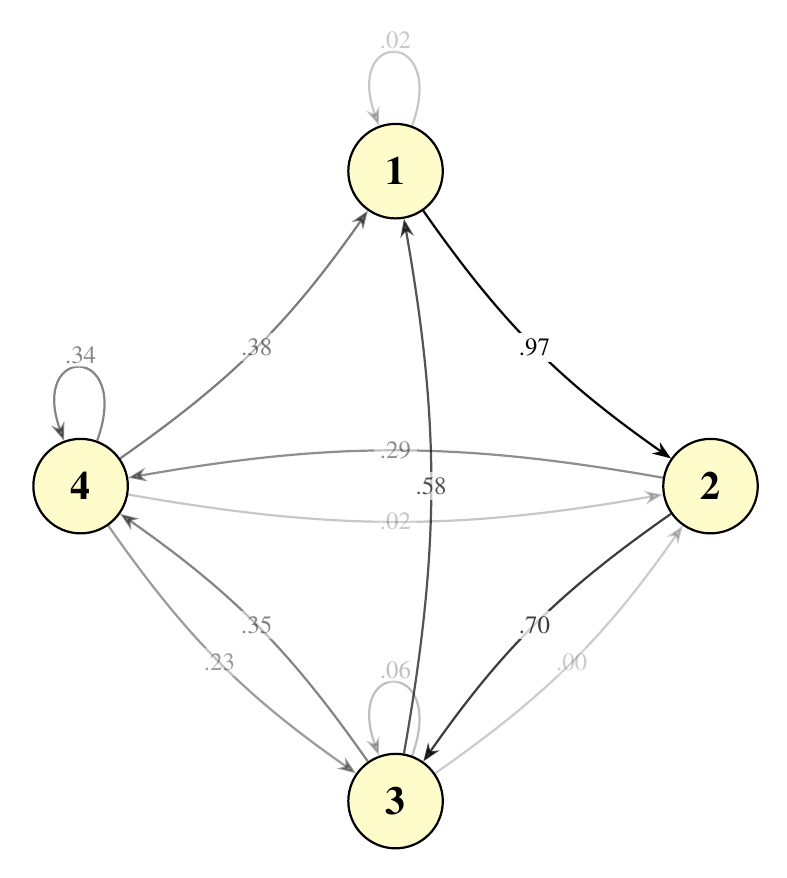
\begin{tikzpicture}[
    node distance=3cm,
    state/.style={circle, draw=black, thick, minimum size=1.2cm, fill=yellow!20, font=\Large\bfseries\fontfamily{ptm}\selectfont},
    every edge/.style={draw, thick, -Stealth},
    edge label/.style={font=\small\fontfamily{ptm}\selectfont, black, fill=white, inner sep=1pt}
]

\node[state] (1) at (90.0:4cm) {1};
\node[state] (2) at (0.0:4cm) {2};
\node[state] (3) at (-90.0:4cm) {3};
\node[state] (4) at (-180.0:4cm) {4};

\path (1) edge[loop, out=70, in=110, looseness=8, opacity=0.22] node[edge label, above] {.02} (1);
\path (1) edge[bend right=10, opacity=0.98] node[edge label, midway, fill=white, inner sep=2pt] {.97} (2);
\path (2) edge[bend right=10, opacity=0.76] node[edge label, midway, fill=white, inner sep=2pt] {.70} (3);
\path (2) edge[bend right=10, opacity=0.44] node[edge label, midway, fill=white, inner sep=2pt] {.29} (4);
\path (3) edge[bend right=10, opacity=0.67] node[edge label, midway, fill=white, inner sep=2pt] {.58} (1);
\path (3) edge[bend right=10, opacity=0.20] node[edge label, midway, fill=white, inner sep=2pt] {.00} (2);
\path (3) edge[loop, out=70, in=110, looseness=8, opacity=0.25] node[edge label, above] {.06} (3);
\path (3) edge[bend right=10, opacity=0.48] node[edge label, midway, fill=white, inner sep=2pt] {.35} (4);
\path (4) edge[bend right=10, opacity=0.51] node[edge label, midway, fill=white, inner sep=2pt] {.38} (1);
\path (4) edge[bend right=10, opacity=0.22] node[edge label, midway, fill=white, inner sep=2pt] {.02} (2);
\path (4) edge[bend right=10, opacity=0.39] node[edge label, midway, fill=white, inner sep=2pt] {.23} (3);
\path (4) edge[loop, out=70, in=110, looseness=8, opacity=0.48] node[edge label, above] {.34} (4);

\end{tikzpicture}
\end{document}
